%%%%%%%%%%%%%%%%%%%%%%%%%%%%%% -*- Mode: Latex -*- %%%%%%%%%%%%%%%%%%%%%%%%%%%%
%% 06-10.tex -- ICSE 2007 submission
%% Author          : Philip Johnson
%% Created On      : Wed Dec 08 2004
%% Last Modified By: 
%% Last Modified On: Wed Sep 20 15:28:37 2006
%% RCS: $Id$
%%%%%%%%%%%%%%%%%%%%%%%%%%%%%%%%%%%%%%%%%%%%%%%%%%%%%%%%%%%%%%%%%%%%%%%%%%%%%%%
%%   Copyright (C) 2002 Philip Johnson
%%%%%%%%%%%%%%%%%%%%%%%%%%%%%%%%%%%%%%%%%%%%%%%%%%%%%%%%%%%%%%%%%%%%%%%%%%%%%%%
%% 

\documentclass[12pt]{article} 
\input{/export/home/csdl/tex/psfig/psfig}
\usepackage{/export/home/csdl/tex/icse2003/latex8}
\usepackage{times}
%% A verbatim-like environment which allows font changes
%%\usepackage{alltt}
%% New LaTeX2e graphics support
\usepackage[final]{graphicx}
% uncomment the % away on next line to produce the final camera-ready version
% and uncomment the \thispagestyle{empty} following \maketitle
\pagestyle{empty}

\begin{document}

\title{Automated software process and product measurement with Hackystat}

\author{Philip M. Johnson \\
\em  Collaborative Software Development Laboratory \\
\em  Department of Information and Computer Sciences \\
\em  University of Hawai'i \\
\em  Honolulu, HI 96822 \\
\em  johnson@hawaii.edu \\
}
\maketitle
\thispagestyle{empty}


\Section{Introduction}
\label{sec:intro}

Most developers, if confronted, would agree that software process and
product metrics have the potential to be useful during development. After
all, many software engineering books have at least one chapter on
metrics for software development, with statements like the following: ``It
is very difficult to evaluate the status or quality of a software
development project and to make objective decisions without accurate,
reliable measurement \cite{Mayrhauser90}.''  Or, as Tom DeMarco 
paraphrases Lord Kelvin,  ``You can't control what you can't measure''
\cite{DeMarco82}.

On the other hand, many of these same developers, if asked if they actually
use software process or products metrics to guide their decision making,
might hesitantly reply with something like the following: ``I would, but
we're a small company and they're too much of hassle to collect.'' Or, ``We
used to have a software process group that did metrics stuff but the group
was eliminated in the last round of budget cuts.''  Or, ``Well, I've heard
that we have a huge database of metric data somewhere, but I'm not sure
what's being done with it.''

One reason why metrics sound good in theory but bad in practice is
cost.  Someone has to collect the data (which is hard), someone has to
analyze it (which is even harder), and someone has to put it in a form in
which developers and managers can interpret it correctly and make useful
decisions from it (which is hardest of all). To address this cost problem,
large organizations often establish a centralized software process group, where
the cost per project can be lessened by amortizing some of the overhead
over multiple projects. Smaller organizations may not have the resources to
support even part-time process people, and thus have to decide whether the
risk of investing in metrics collection and analysis is worth the potential
pay-off.

A second reason why metrics why metrics sound good in theory but bad in
practice is risk.  The high cost of metrics would be an easier pill to
swallow for an organization if the collected data could be guaranteed to
reduce costs down the road; in other words, if metrics was an investment of
resources with low risk and a high rate of return.  The literature
certainly provides evidence that some organizations obtain a significant
payoff from their investment in metrics.  On
the other hand, an organization embarking on a metrics program must
consider risk factors associated with both collection and analysis. One example
of collection risk is a project that is cancelled mid-stream, and thus
renders all of the metrics collected for that project useless.  There are
also a variety of analysis risks. For example, in order for metrics from a
previous project to provide decision-making value a future project, the two
projects must typically be alike in many important ways. What about a
company that switches from C++ to Java?  Or from servlet-based development
to Ruby on Rails? Might that render most, if not all of their previously
collected metrics useless?

This combination of high cost and high risk can go a long way to explaining
why case studies of successful metrics application typically occur in large
organizations: they have both the resources to cover the cost, as well as
the ability to assume the risk of failure.  Of course, when metrics are
collected and analyzed successfully, the results can be spectacular.  For
example, verification activities in Space Shuttle software development
proceed until the number of defects found in a new module match the
predictions based upon the collected metrics.
\cite{Fishman96}.

While this view of metrics cost and risk might appear depressing, it's not,
because it also reveals that cost and risk are tied together: if we can
radically reduce the cost of metrics collection and analysis, then the risk
should be reduced as well.  By analogy, people who enjoy movies sometimes
decide to not pay full price to see a movie of questionable interest in a
theater. However, they might be happy to rent it on DVD, thus lowering the
risk by lowering the cost.  Might there be a way to radically reduce the
cost of software engineering metrics collection and analysis and therefore
its risks, thus making metrics more accessible to more organizations?

\section{Hackystat}

Since 2001, we have been working on the Hackystat Project
(http://www.hackystat.org), an open source approach to lowering
the cost and thus the risk of software engineering product and process
metrics collection and analysis.  Hackystat accomplishes this by providing
a set of software sensors that are attached to developer tools, such as the
editor, the configuration management system, the bug tracking system,
testing system, and so forth.  These sensors unobtrusively gather raw data
about development events and send it off to a central server, where the
data is gathered, analyzed, and made available to developers and managers.
If a user is working offline, sensor data is written to a local log file to
be sent when connectivity can be re-established.

Project members can log in to the web server to see the collected
raw data and run analyses that integrate and abstract the raw sensor
data streams into telemetry.  Hackystat also allows project members to
configure ``alerts`` that watch for specific conditions in the
sensor data stream and send email when these conditions occur. Figure
\ref{fig:architecture} illustrates the basic architecture of the system. 

\begin{figure*}[ht]
  \centering
  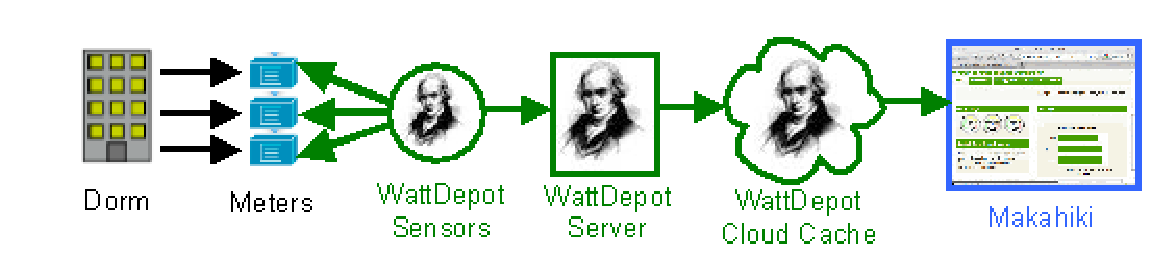
\includegraphics[width=0.60\textwidth]{architecture.eps}
  \caption{The basic architecture of Hackystat.}
  \label{fig:architecture}
\end{figure*}

The set of client-side sensors is extensible and currently includes support
for IDEs (Eclipse, Emacs, JBuilder, Vim, Visual Studio), testing (JUnit,
CppUnit, Emma), build (Ant, Make), configuration management (CVS,
Subversion), static analysis (Checkstyle, FindBugs, PMD), bug tracking
(Jira), size metrics for over twenty five programming languages (SCLC,
LOCC, CCCC), and management (Microsoft Office, OpenOffice.org).

On the server side, an extensible set of analysis modules process the raw
sensor data to create higher-level abstractions.  Over the past five years,
we have implemented a number of different analysis modules to investigate
various issues in software development research and management.  For
example, the Software Project Telemetry module provides support for trend
analysis of multiple sensor data streams to aid in-process decision-making
\cite{csdl2-04-11}, the Zorro module provides support for automated
recognition of Test Driven Development \cite{csdl2-06-02}, the MDS module
provides support for build process analysis for NASA's Mission Data System
project \cite{csdl2-03-07}, the HPC module supports analysis of high
performance computing software development \cite{csdl2-04-22}, the CGQM
module provides a ``continuous'' approach to the Goal-Question-Metric
paradigm \cite{csdl2-05-09}, and the Course module supports software
engineering education \cite{csdl2-03-12}.

At the Hackystat website, http://www.hackystat.org, we provide a set of
``shrinkwrapped'' configurations of the Hackystat modules, including a
``standard'' configuration that contains a basic set of sensors and
analyses most suitable for an organization wishing to evaluate Hackystat.
However, organizations are also free to build custom configurations from
any of the publically distributed modules, or even build their own
proprietary analyses and sensors that they include in their own local
installation of Hackystat.

\section{Daily Project Details}

A very simple example of the way in which Hackystat can be applied in a
project setting is the analysis called ``Daily Project Details''. This
analysis retrieves all of the sensor data associated with the Project 
for a given day and produces a snapshot of the state of the Project 
on that particular day.  Figure \ref{fig:dpd} illustrates the 
``Summary'' window of this analysis for a sample Project.  

\begin{figure*}[t]
  \centering
  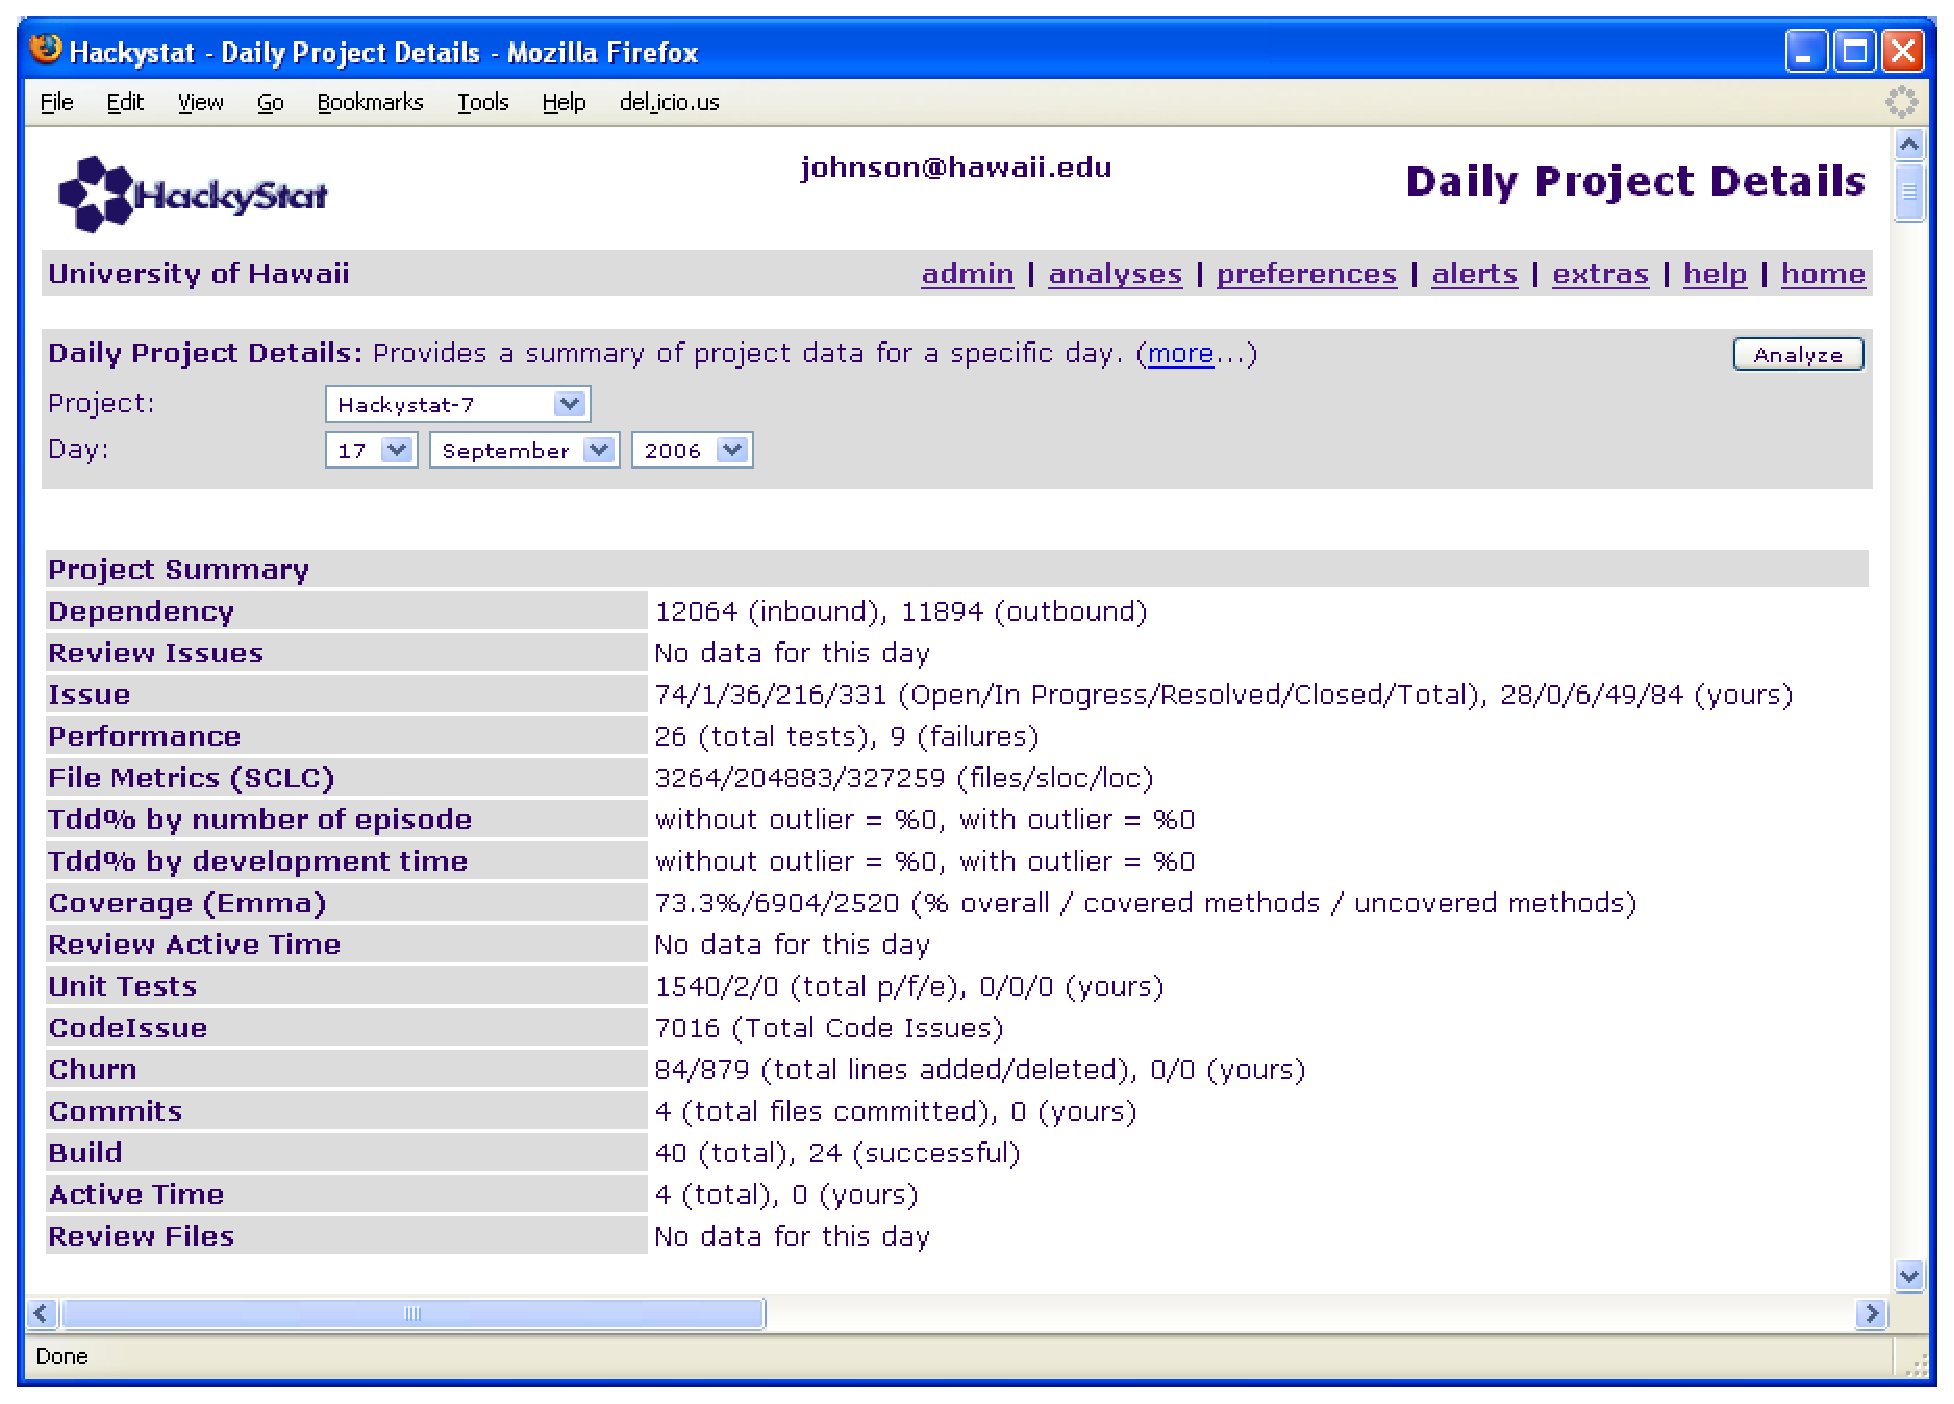
\includegraphics[width=0.60\textwidth]{dpd.eps}
  \caption{The Summary section of the Daily Project Details analysis}
  \label{fig:dpd}
\end{figure*}

The analysis provides process information, such as the ``Active Time''
spent by developers editing code during that day, the number of builds
attempted, and the unit testing invocations and results.  It also provides
product information, such as the size of the system and the number of
dependencies.  Following the Summary section is a set of DrillDowns for
each metric the provide more detailed information.  Figure
\ref{fig:dpd.drilldown} illustrates a portion of one such drilldown for
size on a per-module basis.

\begin{figure*}[t]
  \centering
  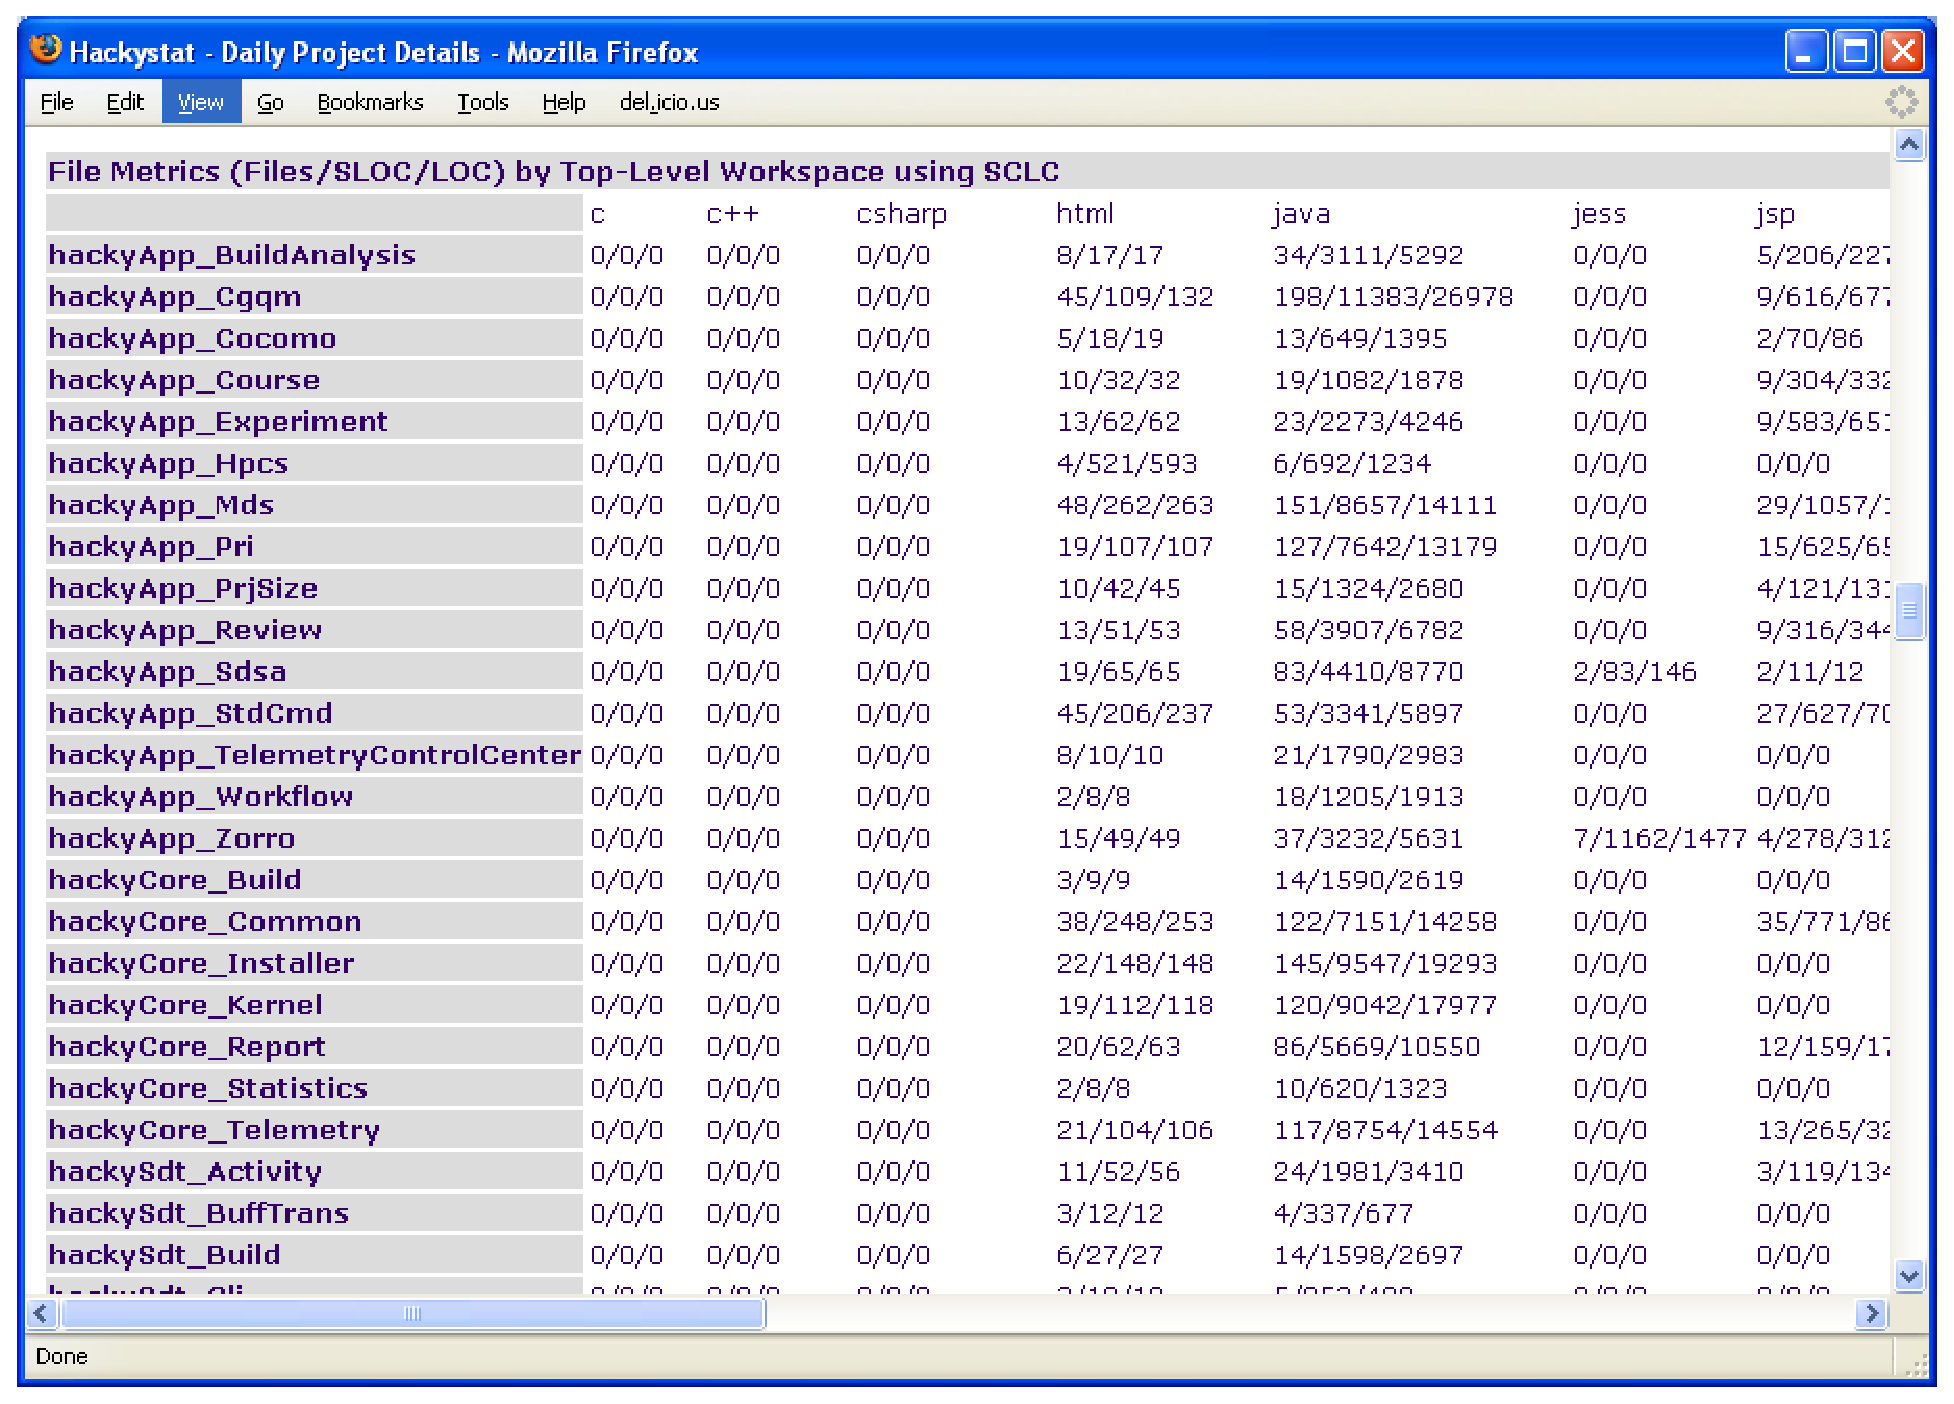
\includegraphics[width=0.60\textwidth]{dpd.drilldown.eps}
  \caption{A Daily Project Details drilldown}
  \label{fig:dpd.drilldown}
\end{figure*}

Daily Project Details can be used in a variety of ways: it helps reveal
what kinds of data is being collected about the system, and what happened
with respect to system development on a previous day.  It provides a window
onto the high-level state of the system that is freely available to all
Project members.  Hackystat includes an ``alert'' for this analysis that
Project members can use to have an email with the summary results for the
previous day sent to them each morning, along with a link to invoke the
analysis if they wish to see the DrillDowns.

\section{Software Project Telemetry}

While the Daily Project Details command provides an interesting snapshot of
the state of development, a natural next question is, ``Well, are these
good numbers or bad numbers?''  Hackystat provides an analysis system
called ``Software Project Telemetry'' to help developers and managers gain
insight into this question by looking at trends in the data for a current project over time. 

For example, one of the product measures that Hackystat can collect is coverage--the 
degree to which the test cases for a system exercise the product code. The Daily
Project Details snapshot above lists the Coverage value as 73.3\%, but is that value
good or bad?  How, in other words, can this metric be made actionable? 

One possible way to evaluate coverage metrics is to monitor trends in the
value over time.  For example, modules whose coverage values are decreasing
significantly over time are probably modules where testing is not keeping
up with new development.  This is actionable information.  Figure
\ref{fig:telemetry} shows a Telemetry chart that shows the three modules
whose coverage has reduced the most over the specified interval in time.
The chart shows that the module represented by the top line,
hackySdt\_Coverage, had a significant decrease in coverage during the five
week period, while the other two ``offenders'' had only slight changes.
The other 70 modules in this system either had increasing coverage during
this time, no change, or else less of a decrease than these three modules.  Thus,
this telemetry chart provides a quick and efficient way to monitor a large
number of modules for developing test case coverage problems. 

\begin{figure*}[t]
  \centering
  \includegraphics[width=0.60\textwidth]{coverage-telemetry.eps}
  \caption{A Software Project Telemetry chart}
  \label{fig:telemetry}
\end{figure*}

The Software Project Telemetry analysis system is designed as a language
for flexible creation of trend-based analyses of arbitrary sensor data, and
can thus accomodate whatever metrics are gathered by an organization.

\section{Inferring Test Driven Design}

The Daily Project Details analysis and Software Project Telemetry are
Hackystat applications that provide insight into Project-level development.
An example of a completely different form of process and product analysis
in Hackystat is the Zorro system for Test Driven Design.  Test Driven
Design is a recent ``agile'' development method that grew out of the Test
First Programming practice in Extreme Programming. The idea, in a nutshell,
is for developers to always write a test case for new or changed
functionality before starting to write the code that implements that
functionality.  TDD has been claimed to naturally generate 100\% coverage,
improve refactoring, provide useful executable documentation, produce
higher code quality, and reduce defect rates
\cite{Beck:03,George:03,Maximilien:03}.  However, different people define TDD 
differently, and it is often hard to know whether people who claim they are doing 
TDD are actually practicing it strictly and without variation. 

To help understand both the definition of TDD and its application in more
detail, we have designed a system called Zorro that gathers process and
product data as developers write Java programs in Eclipse, and then applies
a rule-based system that analyzes the sequence of developer behaviors,
partitions them into ``episodes'', and then classifies them as either TDD
or not TDD depending upon the rules.  Figure \ref{fig:tdd} illustrates a Zorro
analysis of a sample project.

\begin{figure*}[t]
  \centering
  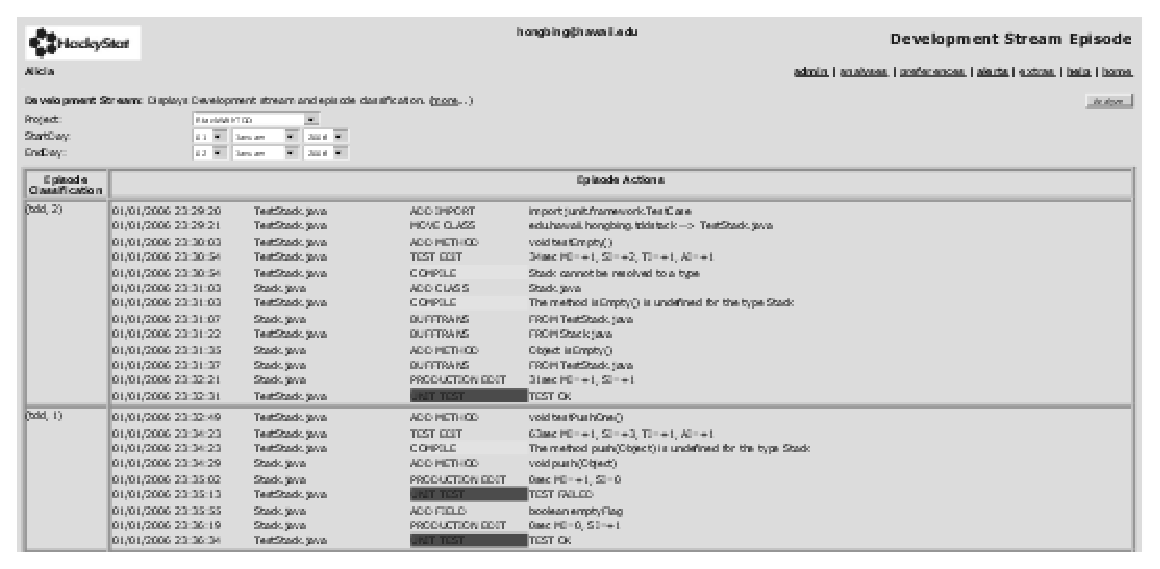
\includegraphics[width=0.90\textwidth]{zorro-interface.eps}
  \caption{Inferring Test Driven Design developer behavior}
  \label{fig:tdd}
\end{figure*}

Zorro is a research project, and so we are trying to understand both if
people do TDD when they say they are doing TDD, as well as understand if
our rule-based system is correctly classifying developer behavior as TDD.
Thus, the interface presents the set of developer events captured by
Hackystat, their division into episodes, their classification as TDD or
non-TDD, an explanation generated by the rule-based system of why the
classification was chosen, and a feedback window that enables developers to
indicate whether they agree with the classification.  Our initial
experiences with Zorro have been encouraging: in a pilot study this Spring,
we found the Zorro correctly classified developer behavior 89\% of the time
\cite{csdl2-06-02}.

\section{Conclusions}

There was a sign is that hung in Albert Einstein's office at Princeton
University: ``Not everything that counts can be counted, and not everything
that can be counted counts''.  It is important to keep this firmly in mind
when embarking on the use of automated software engineering process and
product measurement with a system like Hackystat. While Hackystat can
substantially reduce the cost and thus the risk of metrics collection, it
is possible to capture metrics with Hackystat that don't matter, as well as
miss information about development process and products that are highly
relevent to decision making.

Measurement ``dysfunction'', which means the counterproductive application
of the data, is also possible.  For example, one of the most easily misused
metrics in Hackystat is ``DevTime'', which analyzes events generated by
developer tools to generate a ``proxy'' metric for the amount of time
devoted during the day to work on a particular project by a particular
developer. While the DevTime metric has some interesting applications, it
is so easily misinterpreted by managers as a metric for ``productivity''
that we encourage many organizations new to Hackystat to not collect it at
all!

Caveats aside, we have found that automated metrics collection with
Hackystat can offer new and interesting insights into the way you do
software engineering.  The community of developers working on the open
source project is vibrant and growing, and we invite you to come and
participate with us in the development of the system.
 
\bibliographystyle{/export/home/csdl/tex/icse2003/latex8}
\bibliography{06-10}
\end{document}
 










